\documentclass[a4paper, oneside]{discothesis}

\usepackage[utf8]{inputenc}
\usepackage[T1]{fontenc}

%%%%%%%%%%%%%%%%%%%%%%%%%%%%%%%%%%%%%%%%%%%%%%%%%%%%%%%%%%%%%%%%%%%%%%%%%%%%%%%%%%%%%%%%%%%%%%%%%
% DOCUMENT METADATA

\thesistype{Master Thesis} % Master's Thesis, Bachelor's Thesis, Semester Thesis, Group Project

\title{\fontsize{18}{22}\selectfont A comprehensive study of the phylodynamics of SARS-CoV-2 in Europe}

\author{Cecilia Valenzuela Agüí}
\email{ceciliav@student.ethz.ch}

\institute{Department of Biosystems Science and Engineering \\[2pt]
Computational Evolution \\[2pt]
ETH Zürich}

% Optionally, you can put in your own logo here
%\logo{\includegraphics[width=0.2\columnwidth]{figures/disco_logo_faded}}

\supervisors{Prof.\ Dr.\ Tanja
  Stadler, Dr. Timothy Vaughan, Sarah Nadeau}

% Optionally, keywords and categories of the work can be shown (on the Abstract page)
%\keywords{Keywords go here.}
%\categories{ACM categories go here.}

\date{\today}

%%%%%%%%%%%%%%%%%%%%%%%%%%%%%%%%%%%%%%%%%%%%%%%%%%%%%%%%%%%%%%%%%%%%%%%%%%%%%%%%%%%%%%%%%%%%%%%%%

\begin{document}

\frontmatter % do not remove this line
\maketitle

\cleardoublepage

\begin{acknowledgements}
	I thank Lorem ipsum dolor sit amet, consetetur sadipscing elitr, sed diam nonumy eirmod tempor invidunt ut labore et dolore magna aliquyam erat, sed diam voluptua. At vero eos et accusam et justo duo dolores et ea rebum. Stet clita kasd gubergren, no sea takimata sanctus est Lorem ipsum dolor sit amet. Lorem ipsum dolor sit amet, consetetur sadipscing elitr, sed diam nonumy eirmod tempor invidunt ut labore et dolore magna aliquyam erat, sed diam voluptua. At vero eos et accusam et justo duo dolores et ea rebum. Stet clita kasd gubergren, no sea takimata sanctus est Lorem ipsum dolor sit amet.
\end{acknowledgements}


\begin{abstract}
    The abstract should be short, stating what you did and what the most important result is.
	\todo[inline]{TODO abstract}
	This project focus on the spatial dynamics of the early spread of SARS-CoV-2 in Europe. We apply a novel approach based on the Multi-type Birth Death phylodynamic model to infer structured population dynamics jointly with between-subpopulation transmission rates from viral genome sequences. The inferred epidemic trajectories for the combined outbreak responsible for the observed sequence data will allow us to better understand the entry into and early spread of SARS-CoV-2 in Europe.

	% The early dynamics of the epidemic in Europe surprised the whole world/ From isolated cases detexcted in some, ina  few weeks we faced an unprecedent epidemic with case numbers and death counts stressing well stalished health infraestructures. Understanding what happened during those first month could prepare us to be less surpred in similar future events. Complex dynamics, typical epi date, case identification and travel history, very likely not all cases reported. Genetic sequences are a valuable source of information than together with popualtion dynamic model could inform us about the firrst steps of the coronavirus in Europe. We have integrated sequence data, flisht data and bayesian inference priors? to infer population trajectories - case counts and migration dynamics between the most relevant countrries at the start of the European pandemic.
\end{abstract}

\tableofcontents

\mainmatter % do not remove this line

\chapter{Introduction}

We have many sources of information, but all of them are imperfect in some aspect. Bayesian phylodynamics incorporates different beliefs and data to get a detailed picture of the epidemic. Genetic sequences as an objective source of information about virus evolution and transmision together with viral phylogenetics, transpotation data and geographic data to understand the dynamics and case counts to guide the magnitutde of the numbers.

We lack absolute numbers of the pandemic time resoluted without reporting issues dependent. We lack understading of the dynamics, from where to where, how often, how long.

We can use travel data as a proxy, or we can incorporate it in a model. Lemey et al. Difference we get absolute numbers, not only the rates. And we use BD model instead of coalescent, better to describe beginning of a epidemic. While due to the complexite and time consuming model we dow scaled to europe and only thhe initial phase with the first countries to experiment relevant sars cov 2 epidemics. 



\chapter{Material and Methods}

\textbf{SARS-CoV 2 genome data set.} 
We create a dataset of 360 genetic sequences from December 2019 to March 8 2020, obtained from publicly available data on GISAID \cite{Shu2017} (accessed on November 2020). We follow the Nextstrain workflow for the curation of the dataset \cite{nextstrain}. Sequences with incomplete collection date, less than 27.000 bases in length or with more than 3.000 unknown bases are omitted. Also, sequences from known clusters of transmission or from the same patient are excluded. The resulting worldwide sequence dataset is aligned with MAFFT. The begining and the end of the alignment are masked respectively by 100 and 50 sequences as well as sites  13402, 24389 and 24390, identified by Nextstrain as prone to sequencing errors.

To focus on the early dynamics in Europe we select sequences from China, origin of the epidemic; France and Germany, the European countries with the earliest cases; and Italy and Spain, the European countries with the biggest outbreaks in March. To take into account the dynamics in other regions of Europe we include a group of 50 sequences from other European countries. We limit our sample of Chinese genomes to sequences until January 23, the starting date of the lockdown in Hubei. 

Due to the large (and unprecendented) number of available genetic sequences for SARS-CoV-2, we need to subsample the alignment. Each sequence is subsampled with a probability equal to the probability of having a reported case in that country the day of sample collection, inversely weighted by the probability of having a sequence in GISAID that day in the country. With this subsampling protocol, we aim to get a constant sampling proportion across the full period for each country. 

This dataset of genetic sequences is the main source of information in our phylodynamic analysis. The goal is to infer the phylogenetic tree, i.e. the evolutionary tree-shaped relationship among the sequences, together with the epidemiological transmission parameters that gave rise to it. These parameters are defined within a population dynamic model and will inform us about the epidemic that the viral genetic sequences come from.

\textbf{The multitype birth death model.} 
To study the early dynamics of SARS-CoV-2 in the European countries, we use a simplified version of the multitype birth-death model described in \cite{Kuhnert2016}, following the analysis in \cite{Nadeau2020}. Birth death models are compartmental population models with high flexibility that describe the process of epidemiological transmission. The stochastic formulation of these models are used in phylodynamic analyses \cite{Stadler2012}. In the multitype version, we consider a structured population in types or subpopulations with characteristic within-subpopulation dynamics and migrations between them. In our case, the subpopulations are the different locations of the samples.

The process starts with one infected host in one of the subpopulations, e.g in subpopulation $i$, who can infect another individual at rate $\lambda_i$, become uninfectious at rate $\mu_i$ by death or recovery, migrate to another deme $j$ at rate $m_{ij}$ or be sequenced at rate $\psi_i$ to become part of the phylogenectic tree. This process depicts the full transmission dynamics and specifically, the generation of the phylogenetic tree that we observed from our sequence data. 

Under this model, we are able to compute the likelihood of the multitype birth-death parameters for a given tree. This likelihood is derived in \cite{Kuhnert2016} by considering the probability of an individual evolved as observed in the tree. This derivation is analogous to the work in \cite{Stadler2013}, which is based on ideas from \cite{Maddison2007}.

We parameterize our model in terms of the effective reproductive number $R_i = \frac{\lambda_i}{\mu_i + \psi_i}$, a key value in epidemic control and understanding, the rate of becoming uninfectious $\delta_i = \mu_i + \psi_i$, the probability of and individual to be sequenced $s_i = \frac{\psi_i}{\mu_i + \psi_i}$ and the migration rates between locations $m_ij$.\\

\textbf{Epidemic trajectories and structured trees.} 
We will refer to the full sequence of transmissions, recoveries/deaths, migrations and sampling events as an epidemic trajectory. One set of sequences, and therefore one phylogenetic tree, is the product of one epidemic trajectory. Moreover, the tree represents a fraction of the events in the epidemic trajectory, those that involve the sampled individuals. In epidemiology, we aim to learn about the true epidemic trajectory since we usually have incomplete information caused by unreported cases or unknown transmission chains.

From the sequences metadata, we know the location of the tree tips. However, if we know the epidemic trajectory we also know the location of the lineage at any point in time in the tree. We will refer to the phylogenies with ancentral locations mapped onto the tree as structured trees \cite{Vaughan2014}. In Fig \ref{fig:epitrajs} we show the epidemic trajectories corresponding to two different subpopulations and the structured tree of a set of samples. The change of ancestral location, represented by a change in color from blue to red in the tree, is caused by a migration event from one subpopulation to the other, depicted in the epidemic trajectories.

\begin{figure}[h]
    \centering
    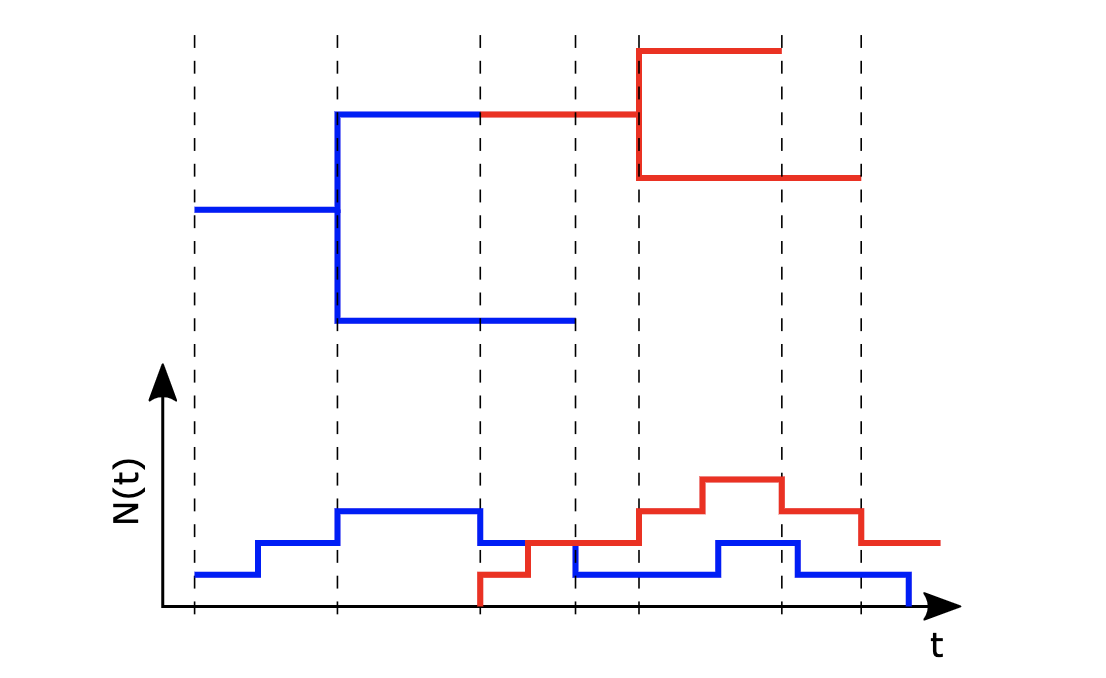
\includegraphics[width=\textwidth]{figures/epitrajs.png}
    \caption{Example of structured tree (up) and epidemic trajectories (bottom) for two types. The horizontal axis represents time, and for the epidemic trajectories the vertical axis is the population size N(t). Figure from Tim Vaughan. \todo[inline]{Use figure from EpinInf paper?}}
    \label{fig:epitrajs}
\end{figure}

\textbf{Bayesian Inference with BDMM-Prime.} 
We want to infer the epidemic trajectories under the multitype birth-death model fit to a set of samples collected throughout SARS-CoV-2 early epidemics in Europe. In order to do this, we have to estimate the joint posterior distribution of the structured tree $\mathcal{T}_c$, the epidemic trajectory $\mathcal{E}$, the substitution model parameters $\theta$ and the multi-type birth death parameters $\eta$. This posterior probability can be expressed with Bayes' formula as:

\begin{equation}
P(\mathcal{T}_c, \mathcal{E}, \theta, \eta | A ) = \frac{P(A | \mathcal{T}_c, \mathcal{E}, \theta, \eta ) P(\mathcal{T}_c, \mathcal{E}, \theta, \eta)}{P(A)}
\label{eq:posterior1}
\end{equation}

where A is the sequence alignment.

We make the following independence assumptions:

\begin{align}
P(A | \mathcal{T}_c, \mathcal{E}, \theta, \eta ) &= P(A | \mathcal{T},\theta )\\
P(\mathcal{T}_c, \mathcal{E}, \theta, \eta) &= P(\mathcal{T}_c|\mathcal{T}, \eta) P(\mathcal{E}|\mathcal{T}_c, \eta) P(\mathcal{T} | \eta ) P(\theta) P(\eta)
\label{eq:assumptions}
\end{align}


Where $\mathcal{T}$ is the rooted time tree without ancestral locations. Thus, we can express Equation \ref{eq:posterior1} in terms of the conditional distributions:

\begin{align}
P(\mathcal{T}_c, \mathcal{E}, \theta, \eta | A) &= P(\mathcal{T}_c|\mathcal{T}, \eta) P(\mathcal{E}|\mathcal{T}_c, \eta) \frac{P(A | \mathcal{T}, \theta) P(\mathcal{T} | \eta) P(\theta) P(\eta)}{P(A)}\\
&= P(\mathcal{T}_c|\mathcal{T}, \eta) P(\mathcal{E}|\mathcal{T}_c, \eta) P(\mathcal{T}, \theta, \eta | A)
\label{eq:posterior2}
\end{align}

$P(\mathcal{T}_c|\mathcal{T}, \eta)$, $P(\mathcal{E}|\mathcal{T}_c, \eta)$ and $P(\mathcal{T}, \theta, \eta | A)$ are the posterior probabilities of the structured tree, the epidemic trajectory and the joint posterior of the phylogenetic tree (without ancestral locations) and the model parameters. The tree likelihood $P(A | \mathcal{T},\theta )$ is the probability of the sequence alignment and can be efficiently evaluated using Felsenstein’s pruning algorithm \cite{Felsenstein1981}. The tree prior, $P(\mathcal{T} | \eta)$ also called phylodynamic likelihood is derived from the multitype birth-death model. $P(\theta)$ and $P(\eta)$ represent our prior belief in the distribution of the population and substitution model parameters. 

We use a Markov chain Monte Carlo (MCMC) Metropolis-Hastings algorihtm to approximate this posterior. Since the MCMC only uses ratios of posterior probabilities, we avoid calculating the marginal likelihood $P(A)$. This algorithm is implemented in BDMM-Prime package \cite{bdmmp} for BEAST 2.6.3 \cite{Bouckaert2019}. BDMM-Prime first samples from $P(\mathcal{T}, \theta, \eta | A)$, then in a second step these samples are augmented by sampling from $P(\mathcal{T}_c|\mathcal{T}, \eta)$ and $P(\mathcal{E}|\mathcal{T}_c, \eta) $ and adding these variables to obtain the overall posterior $P(\mathcal{T}_c, \mathcal{E}, \theta, \eta | A)$. In this way, $P(\mathcal{T}_c|\mathcal{T}, \eta)$ and $P(\mathcal{E}|\mathcal{T}_c, \eta) $  are only calculated for a subset of samples instead of every MCMC step.


While it is also possible to include $\mathcal{T}_c$ and $\mathcal{E}$ directly into the Bayes' rule as implemented in EpiInf package \cite{Vaughan2019}, the factorization of the posterior in these three terms allow us to use the standard birth-death-sampling tree prior implementations in BDMM to compute $P(\mathcal{T}, \theta, \eta | A)$ \cite{Kuhnert2016} \cite{Scire2020}. This will speedup the analysis with almost no overhead compared to the standard BDMM inference and can be used in pre-existing multitype analyses withoud additional MCMC.\\

\textbf{Stochastic mapping of ancestral locations and epidemic trajectories}
To sample from $P(\mathcal{T}_c|\mathcal{T}, \eta)$, BDMM-Prime implements a stochastic mapping algorithm based on the work by \cite{Hohna2019}. A set of differential equations is numerically integrated over $\mathcal{T}$ to obtain the marginal probability of a location value at any point along each branch. From this probabilities, we can derive time-dependent rates that define the changes of the location along the tree according to a continuous-time Markov process. Then, we can simulate forward in time from the root of the tree the location trajectories down the tree edges. For a detailed derivation of the stochastic mapping of the algorithm refer to \cite{VaughanWIP}.\\

In the case of $P(\mathcal{E}|\mathcal{T}_c, \eta)$, following Bayes'rule:

\begin{equation}
P(\mathcal{E}|\mathcal{T}_c, \eta) = \frac{P(\mathcal{T}_c, \eta|\mathcal{E}) P(\mathcal{E})}{P(\mathcal{T}_c, \eta)} = \frac{P(\mathcal{T}_c|\mathcal{E}) P(\mathcal{E}| \eta)}{P(\mathcal{T}_c | \eta)}
\label{trajectories}
\end{equation}

We can easily compute the probability of a structured tree for a given epidemic trajectory $P(\mathcal{T}_c|\mathcal{E})$ as described in \cite{Vaughan2019}. Each node in the structured tree must correspond to a compatible event in the epidemic trajectory for this probability to be nonzero. If we simulate an epidemic trajectory directly from $P(\mathcal{E}| \eta)$, it is very likely that the simulated events will not match with the events in the tree and $P(\mathcal{T}_c|\mathcal{E})$ will be 0. To avoid this problem, we simulate from $P^*(\mathcal{E}| \eta)$, which guarantees trajectories with non-zero probabilities by enforcing the tree events. Provided we weight these trajectories accordingly we can efficiently sample from $P(\mathcal{E}|\mathcal{T}_c, \eta)$:

\begin{equation}
P(\mathcal{E}^{(a)}|\mathcal{T}_c, \eta) = w_a^* P^*(\mathcal{E}^{(a)}| \eta) \propto P(\mathcal{T}_c | \mathcal{E}^{(a)}) \frac{P(\mathcal{E}^{(a)} | \eta)}{P^*(\mathcal{E}^{(a)} | \eta)} P^*(\mathcal{E}^{(a)}| \eta)
\label{eq:traj}
\end{equation}

The epidemic trajectories are simulated with an adaptive tau-leaping algorithm \cite{Gillespie2000} in BDMM-Prime. This method is based on the Gillespie algorithm \cite{Gillespie1977} but the simulation time is divided in small intervals and the number of events is drawn from a poisson distribution for each interval. This algorithm is more efficient that Gillespie when we have a high number of individuals since we have to update the rates less often. 

We simulate a fixed number of trajectories, called particles, for each set of population parameters $\eta$ and structured tree $\mathcal{T}_c$. The trajectories are simulated until some point and are weigthed as described in Equation \ref{eq:traj}. We resample using importance sampling to get rid of low-weighted trajectories and then resume the simulation of all the particles from the sampled trajectory ending point. This process is repeated until the end of the simulation. Then, we sample one single trajectory from the set of final trajectories with important sampling and record each event and its timing to future analysis \cite{VaughanWIP}. All these steps are implemented by BDMM-Prime trajectory logger and we use it in our analysis.\\

We conducted two different analyses. One with constant migration rates as in the standard multi-type birth death model and the other one with time-changing migration rates informed by travel data. We use the BDMM-Prime package \cite{bdmmp} implemented in BEAST 2.6.3 \cite{beast}. We run 10 parallel chains for analysis, of $10^7$ iterations each with different initial values. These chains are assesed for convergence using Tracer v.1.7.1 and then combined after removing a 10\% burnin. We check that the effective sample size (ESS) is greater than 200 for all parameters. The stochastic mapping of structured trees and epidemic trajectories is performed in a second step using the trace and tree logs from the MCMC. We use 300, 1000, 3000 and 10000 particles in the tau-leaping simulation of epidemic trajectories, and a tolerance of 0.03 for selecting tau leap length.\\


\textbf{Incorporating air travel data and geographic distances.}
 In order to inform our migration rates with external information, and to avoid having to estimate a large number of migration rates we implement a generalized linear model (GLM) for the migration matrix based on \cite{Lemey2014} and \cite{Nicola2019}. This GLM model parametrizes the migration rates as a log linear function of a number of potential predictors, Equation \ref{eq:glm}. For each predictor $x_i$, the GLM parameterization includes a coefficient $\beta_i$, which quantifies the effect size of the predictor, and a binary indicator variable $\delta_i$, that allows the predictor to be included or excluded from the model. The parameter $c$ represents the overal magnitude of migration. This means that if every indicator is 0, every migration rate will be equal to this parameter. In the MCMC, we estimate the effect size of each of the predictors, as well as their inclusion probability $\mathbb{E}[\delta_i]$.

\begin{equation}
m_{ij} = c \exp(\sum_{i = 1}^p \delta_i \beta_i xij)
\label{eq:glm}
\end{equation}

In a similar way to the GLM formulation in \cite{Lemey2020} we consider as predictors air travel data and geographical distance between locations. We define three time periods in our analysis: from the origin of the epidemic to January 23 (Hubei lockdown), from January 23 to end of February, from March 1 to March 8. The international travel during these months decreased drastically due to the increasing awareness about the SARS-CoV-2 pandemic as is shown in Figure \ref{fig:travel}. Thus, we would expect the migration rates to change during the time of the analysis. 

The air travel data is obtained from EUROSTATS transport datasets \textit{avia\_paexcc} and \textit{avia\_paincc}, in particular the passengers carried departures values for December 2019, January, February and March 2020. We compute the average daily flux of passengers for each of the time periods. The geographical distance is defined as the great circle pairwise distance between the centroids of the countries, computed based on the Natural Earth project (the 1:50m resolution version) world map 2013. The predictors are log transformed, a pseudocount is added to make all values positive, and then they are standardized, following the description in \cite{Lemey2014}.

\begin{figure}[h]
    \centering
    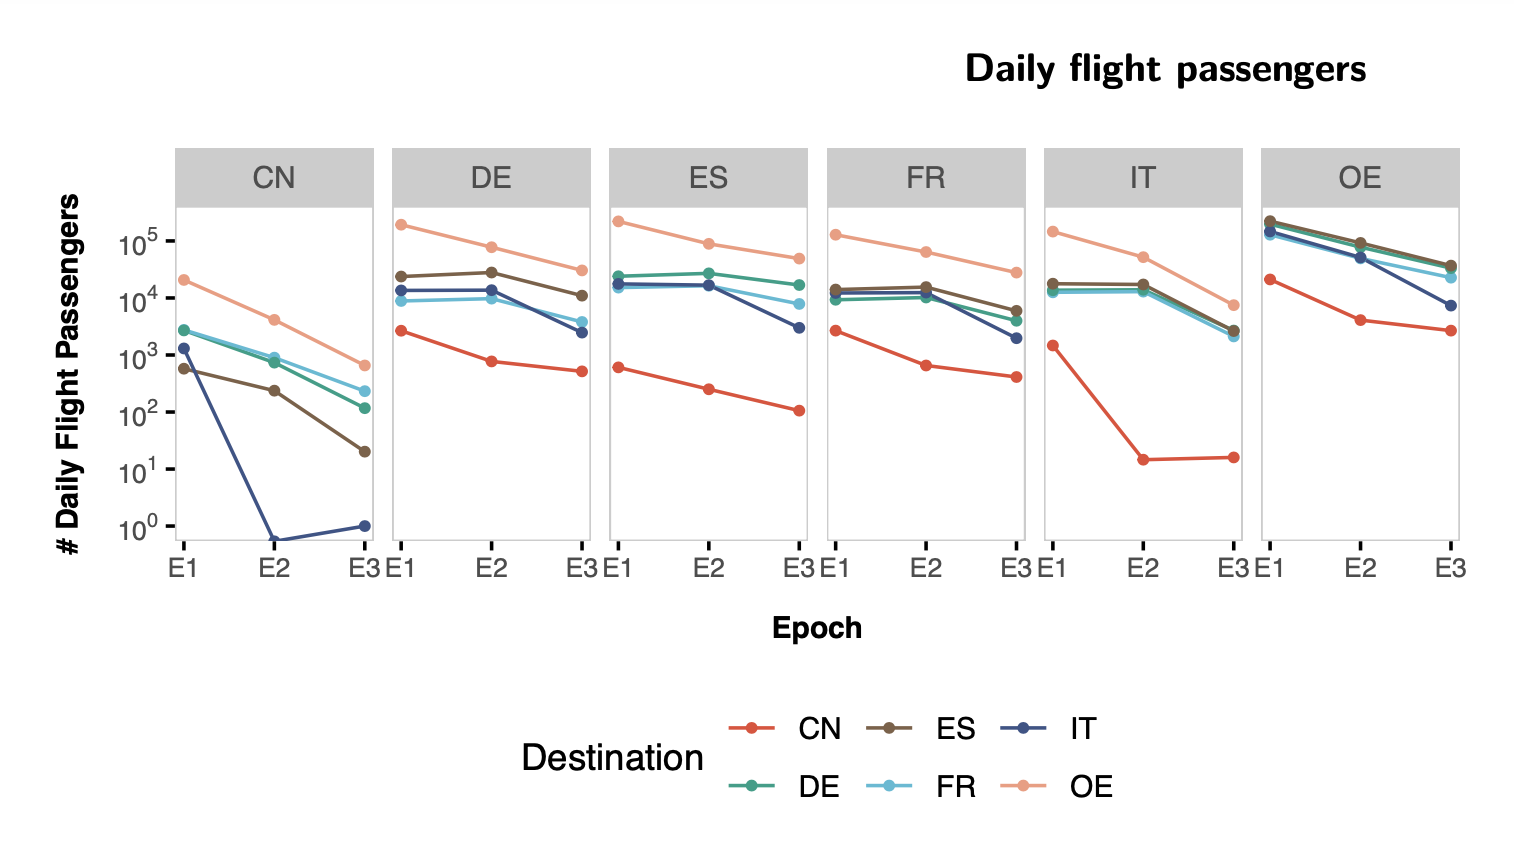
\includegraphics[width=\textwidth]{figures/flight_data.png}
    \caption{\todo[inline]{improve figure}}
    \label{fig:epitrajs}
\end{figure}

\textbf{Model specifications and priors.} 
Since we focus on the early epidemic outbreak, we expect un unimpeded spread of the virus that can be described by the exponential growth of the infected population and no significant decrease in the number of susceptibles over time \cite{Boskova2014}. Thus, we assume a constant basic reproductive number $R_0$ for each of the European countries before the lockdown in the Lombardy region in March 8. However, in China the first wave of the epidedmic had almost concluded in March so we can not make the same assumption. We fixed the reproductive number in China and include three different periods, changing on January 23 and February 10 based on \cite{Pan2020} \cite{Wu2020} \cite{Xiao2020}. Before January 23, we use the estimation in \cite{Park2020} \cite{Billah2020} to fix the basic reproductive number $R_0$ in China to $2.9$ . From January 23 to February 10 and from February 11 to March 8, we calculate the average effective reproductive number based on the estimations in \cite{covidre} \cite{Huisman2020} and obtain the $R_e$ in China to be $1.1$ and $0.43$ respectively.   

In Table \ref{table:priors} we show the values and prior distributions used in the Bayesian inference of the multitype birth death model and substitution parameters. Several of these model specifications are identical to those from \cite{Nadeau2020}.

\renewcommand{\arraystretch}{1.2}
\begin{table}[h]
\footnotesize
\begin{tabular}{@{}lll@{}}
\toprule
\textbf{Parameter}  & \textbf{Value or Prior} & \textbf{Rationale}                                              \\ \hline
\begin{tabular}[c]{@{}l@{}}Nucleotide substitution \\ model\end{tabular} &
  HKY + Gamma &
  \begin{tabular}[c]{@{}l@{}}Unequal transition/transversion rates, \\ unequal base frequencies, rate\\ heterogeneity among sites with 4 categories\end{tabular} \\
Clock rate          & 0.0008                  & Approximatelly 24 mutations per year \textbackslash{}cite\{10\} \\
Location of origin  & Hubei                   & Putative pandemic origin                                        \\
Time of origin      & Lognormal (-1, 0.2)     & \begin{tabular}[c]{@{}l@{}}Median 26 October, 95\% IQR 22 August \\ to 8 December 2019 \end{tabular}       \\
\begin{tabular}[c]{@{}l@{}}European countries \\ reproductive number\end{tabular} &
  Lognormal (0.8, 0.5) &
  Median 2.2, 95\% IQR 0.8 to 5.9 \\
\begin{tabular}[c]{@{}l@{}}China reproductive \\ number\end{tabular} &
  \begin{tabular}[c]{@{}l@{}}Origin - Jan 23: 2.9\\ Jan 23 - Feb 10: 1.1\\ Feb 11 - Mar 8:  0.43\end{tabular} &
  Fixed based on \textbackslash{}cite\{\}. \\
\begin{tabular}[c]{@{}l@{}}Becoming uninfectious \\ rate \end{tabular} &
  36.5 y-1 &
  \begin{tabular}[c]{@{}l@{}}Period between infections and becoming \\ uninfectious assumed exponentially \\ distributed with a mean of 10 days\end{tabular} \\
Sampling proportion &                         & Upper bounds based on reported cases:                           \\
China               & Uniform (0, 0.12)       &                                                                 \\
France              & Uniform (0, 0.07)       &                                                                 \\
Germany             & Uniform (0, 0.07)       &                                                                 \\
Italy               & Uniform (0, 0.01)       &                                                                 \\
Spain               & Uniform (0, 0.08)       &                                                                 \\
Other European      & Uniform (0, 0.03)       &                                                                 \\
Sampling start date & December 23, 2019       & Just before first sample from China                             \\
\begin{tabular}[c]{@{}l@{}}Sampling end date \\ (only China)\end{tabular} &
  January 23, 2020 &
  \begin{tabular}[c]{@{}l@{}} Only included Chinese sequences before \\ Lockdown in Hubei \end{tabular} 		\\ 

\begin{tabular}[c]{@{}l@{}}Migration rates \\ (no GLM analysis)\end{tabular} & Lognormal(0,1) & Median, IQR                            \\
\begin{tabular}[c]{@{}l@{}}Migration rates \\ (GLM analysis)\end{tabular} & Uniform(0,50) & \begin{tabular}[c]{@{}l@{}}7.3 days as mean of exponential time \\ to travel for every individual \end{tabular}\\
\begin{tabular}[c]{@{}l@{}}Migration rates \\ change times \\(GLM analysis)\end{tabular} & December 23, 2019 and March 1, 2020       & \\
\begin{tabular}[c]{@{}l@{}}Global scaler \\ GLM parameter\end{tabular} & December 23, 2019 & Median, IQR                              \\
\begin{tabular}[c]{@{}l@{}}Coefficients \\ GLM predictors\end{tabular} & Normal (0, 2) & Median 0, IQR                            							\\
\begin{tabular}[c]{@{}l@{}}Binary indicators \\ GLM predictors\end{tabular} & 0 - 1 equiprobable & BitFlipOperator.  			\\

\bottomrule
\end{tabular}
\caption{Caption \todo[inline]{finish table and caption}}
\label{table:priors}
\end{table}

\textbf{Data availability.}
The SARS-CoV-2 genetic data can be downloaded from www.gisaid.org \cite{Shu2017}. Supplementary Table \ref{stable:seqs} \todo{todo} lists accession numbers for the genetic sequences used in this study. Reported SARS-CoV-2 case counts are obtained from the country official agencies indicated in Table \ref{table:cases} \todo{todo}. Flight data can be obtained from EUROSTATS https://ec.europa.eu/eurostat/.

\textbf{Code availability and analyses reproducibility.}
All the code is available at ...
To ensure the reproducibility of the analysis, we have implemented the whole workflow with Snakemake \cite{snakemake}. The workflow is a modified version of Nextrain workflow \cite{nextstrain} with the additional rules for BEAST 2 analysis and results processing. 



\chapter{Results}

\textbf{The origin of SARS-CoV-2 in Europe} 
While the first cases in Europe were reported end of January, the first European wave is suspected to have started earlier but been undetected, mistaken for other common repiratory diseases in winter. In our model, we assume the origin of SARS-CoV-2 in Europe to be an imported case from China into any of the European countries. We analyze the time and destination of the first imported case in the infered epidemic trajectories and estimate the origin of the European epidemic on January 2020 ($95\%$ CCI). As shown in Figure \ref{fig:firstEUcase} A, we place the destination country of this first imported case in Italy or France, with x of probability each.  

Likewise, we analyze the first ten imported cases into Europe and obtain the probability distribution of the source and destination country, Figure \ref{fig:firstEUcase} B and C.  The role of Italy as the receptor of these firts cases is highlighted even more looking at several cases. Earlly introductions in Spain have a very low probabilty, looking like Spain was not a key player in the orrigin of SARS-CoV-2 in Europe. China is the main source of these first introductions, supporting the hypothesis of the European epidemic seeded by several and not just one imported cases from China.

\begin{figure}[p]
    \centering
    \includegraphics[width=\textwidth]{210205_europe10_figtraj0405.png}
    \caption{First introductions of SARS-CoV-2. From the set of random subsampled trajectories, the first introduction time for each epidemic trajectory is recorded and the probability distribution over all these times is plotted. \textbf{A} Probability density of the time of first introduction for each deme. Each dotted line represents the first date when cases where reported to ECDC by deme color. In the case of China, the distribution of the origin time is plotted, since in the analysis we defined Chine as the origin of the epidemic with probability 1. For the other five demes, the distribution of the time of first migration into the deme is shown. \textbf{B} Stacked probability density of the destination of first introduction into Europe coloured by the destination deme. This first case corresponds to the first migration event from China to any of the European countries. \textbf{C} Stacked probability density of the source of the first introduction for each deme coloured by the source deme of the introduction.}
    \label{fig:firstEUcase}
    \todo[inline]{ticks for every month}
\end{figure}


\textbf{The early spread of SARS-CoV-2 among the European countries}


Since in our model we consider the different European countries, we can also estimate from the infered epidemic trajectories the origin of the epidedmic in each particular country. In Figure we have the origin time for each country compared to the ddate of the first reporrted case to ECDC by that country. In average, we predict a delay in detection of x days for the Eurropean countries, out of the $95\% CCI$ for France, Germany and Italy. Origin in Spain close to the official detection day. We estimate that the epidemic in any of the European countries was seeded by an imported case from China as seen in Figurem with some small prrobability for Germany and Italy of having orriginatetdd from a case from each other, and mostly half of the rpobability in the case of Spain from the epidemdic started with a case imported from one of the others Euroopean countries. Same than before, we can look into the first 10 imported cases into each country and now we see that the transmission between european countries adquire much moer importance,  so once SARS-CoV-2 entered Europe, the transmission between european countrries were soon more important than the cases coming from China. This coulld relate also to the decrease in tthe trravel to and from China seen in figure.

Among the European countries, France and Germany have the earlier time of introduction, followed by Italy, Other European deme and Spain. We can compare this inferred dates of introduction with the day each country reported its first case to ECDC. In all cases, the reported day was later than the median of the inferred distribution, but it is inside the 95\% interval.\\

The first case in each European country could have been imported from China or from other European country with an ongoing epidemic that started earlier. However, in our analysis we obtain a much higher support for China being the most probable source of the first case for all European demes, Figure \ref{fig:first} C.\\

Even if the first case in each European country came from China, the timing of the introductions in the European countries relative to each other probablu expanded across several days, defining and order of countries with the time of their first case. 

We can analyze if this order of countries, defined by the time in which the first case occured, is shared among the majority of the inferred population trajectories, Figure \ref{fig:first_imig}. We obtain that the first European country with a SARS-CoV-2 case was more likely France or Germany, followed by Italy and Other European deme. While Spain was more likely the last European country with a case among the ones included in the analysis.\\

\begin{figure}[ht]
    \centering
    \includegraphics[width=\textwidth]{210205_europe10_figtraj06.png}
    \caption{Countries ordered by the time of its first introduction, i.e. first case in the country. Each row is the order for one of the subsampled epidemic trajectories and each column represents the position relative to the other countries first introduction, e.g. in first position for all epidemic trajectories is China since it is the origin of the epidemic.} 
    \label{fig:first_imig}
\end{figure}

Along the same lines, we could ask if this order of countries is mantained when instead of looking at the first case in the country we look into at first case exported (migration) from that country to other European country. In Figure \ref{fig:first_omig} we observe a similar pattern to the first cases order, with Germany, France and Italy being the countries in the first positions in more than half of the inferred trajectories and never in the last position, and Spain as the country in last position in almost every epidemic trajectory.\\

\begin{figure}[ht]
    \centering
    \includegraphics[width=\textwidth]{210205_europe10_figtraj07.png}
    \caption{Order of countries by the time of its first migration out of the country, i.e. first exported case to other country. Each row is the order for one of the subsampled epidemic trajectories and each column represents the position relative to the other countries first migration, e.g. in first position for all epidemic trajectories is China since it was the first country with exported cases of SARS-CoV-2 to other regions.}
    \label{fig:first_omig}
    \todo[inline]{I don't like much these "order" plots but maybe they could be useful to detect interesting patterns?}
\end{figure}

\textbf{Detection timing and response to the European epidemics}


\begin{figure}[p]
    \centering
    \includegraphics[width=\textwidth]{210205_europe10_figtraj03.png}
    \caption{First introductions of SARS-CoV-2. From the set of random subsampled trajectories, the first introduction time for each epidemic trajectory is recorded and the probability distribution over all these times is plotted. \textbf{A} Probability density of the time of first introduction for each deme. Each dotted line represents the first date when cases where reported to ECDC by deme color. In the case of China, the distribution of the origin time is plotted, since in the analysis we defined Chine as the origin of the epidemic with probability 1. For the other five demes, the distribution of the time of first migration into the deme is shown. \textbf{B} Stacked probability density of the destination of first introduction into Europe coloured by the destination deme. This first case corresponds to the first migration event from China to any of the European countries. \textbf{C} Stacked probability density of the source of the first introduction for each deme coloured by the source deme of the introduction.}
    \label{fig:first}
    \todo[inline]{ticks for every month}
\end{figure}


The time between the first case in the country, i.e. first incoming migration event and the first case from within-region transmission is of x  (y-z) with similar values for all demes?. The time from the first incoming migration to the first outgoing migration is longer with a median of x (y-z). (This could be interesting to say if we should focus or not the screening and testing capacities to detect incoming migrations or if when we have evidence of cases in the population we shoud follow a more general strategy to find cases in the population according to the model. Is it different for each country?)\\

(How well did the countries detecting the first cases, there were already within region transmision?) We compare the date of the first reported rate of each country with the date in which within-region transmission for that country started according to the model. We see some differences among countries, France and Germany had in all inferred epidemic trajectories ongoing within-region transmission when first cases werre reported, while x\% of epidemic trajectories did not have had a within region transmission case when the first case in Spain was reported.\\


\begin{figure}[p]
    \centering
    \includegraphics[width=\textwidth]{210205_europe10_figtraj13.png}
    \caption{First introductions of SARS-CoV-2. From the set of random subsampled trajectories, the first introduction time for each epidemic trajectory is recorded and the probability distribution over all these times is plotted. \textbf{A} Probability density of the time of first introduction for each deme. Each dotted line represents the first date when cases where reported to ECDC by deme color. In the case of China, the distribution of the origin time is plotted, since in the analysis we defined Chine as the origin of the epidemic with probability 1. For the other five demes, the distribution of the time of first migration into the deme is shown. \textbf{B} Stacked probability density of the destination of first introduction into Europe coloured by the destination deme. This first case corresponds to the first migration event from China to any of the European countries. \textbf{C} Stacked probability density of the source of the first introduction for each deme coloured by the source deme of the introduction.}
    \label{fig:first}
    \todo[inline]{ticks for every month}
\end{figure}


We can also compare the date of the first reported case with the date of the first outgoing migration from the country. (This could be interesting to say if a extreme measure closing borders with the first case could be effective to impede transmission to other countries: percentage of trajectories whre transmission to Europe would have been avoided. For other countries we can look at how many migrations events could have been avoided (and how many not) if the country closed borders after first reported case according to the model. Not realistic measure, extreme case.)\\ 


\textbf{Burden of SARS-CoV-2 infections in Europe}
The inferred epidemic trajectories contain the information about the total number of cases until 8th of March. For the European countries, we obtain an inferred number of total cases above the number of confirmed cases to ECDC, consistent with known limited test availability of the first wave and  previous studies results \cite{Li2020} \cite{Wu2020}. These cases counts correspond to \todo{Include values} x-y times higher than the number of reported cases. Italy is the country with the highest infered number of cases x, followed by Spain, France and Germany. The infered number of cases for China is below the reported number of cases. \todo{limitations of the model, sequence information, partial outbreak dynamics}\\


\begin{figure}[ht]
    \centering
    \includegraphics[width=0.8\textwidth]{210205_europe10_figtraj01.png}
    \caption{Inferred population size summary statistics for each deme over time. The line represents the median population trajectory and the interval is the 95\%  credible interval in log scale from a random subsampled set of inferred epidemic trajectories.}
    \label{fig:gribbon}
    \todo[inline]{Specify that the random subset are 500 trajectories in all figure legends}
\end{figure}


\begin{figure}[p]
    \centering
    \includegraphics[width=0.9\textwidth]{210205_europe10_figtraj02.png}
    \caption{Inferred epidemic trajectories over time. A random subsampled set of 500 trajectories is plotted. In each subplot, the trajectories (solid lines) are compared with the ECDC cumulative case count data (dashed line) in log scale.}
    \label{fig:trajs}
\end{figure}


In Figure \ref{fig:gribbon} and/or \ref{fig:trajs} we compare the total number of inferred cases by day to the total cumulative number of cases that have been reported to ECDC that same day. Our inferred case counts follow a exponential growth earlier in time than the reported curve and with higher number of cases, being the difference bigger for later times in the epidemic.\\


\begin{figure}[ht]
    \centering
    \includegraphics[width=0.9\textwidth]{210205_europe10_figtraj11.png}
    \caption{5-days reporting rate, calculated as the cumulative number of ECDC reported cases by the median number of cumulative inferred cases in intervals of 5 days until 8th of March. }
    \label{fig:reported}
\end{figure}


\begin{figure}[p]
    \centering
    \includegraphics[width=\textwidth]{210205_europe10_figtraj12.png}
    \caption{First introductions of SARS-CoV-2. From the set of random subsampled trajectories, the first introduction time for each epidemic trajectory is recorded and the probability distribution over all these times is plotted. \textbf{A} Probability density of the time of first introduction for each deme. Each dotted line represents the first date when cases where reported to ECDC by deme color. In the case of China, the distribution of the origin time is plotted, since in the analysis we defined Chine as the origin of the epidemic with probability 1. For the other five demes, the distribution of the time of first migration into the deme is shown. \textbf{B} Stacked probability density of the destination of first introduction into Europe coloured by the destination deme. This first case corresponds to the first migration event from China to any of the European countries. \textbf{C} Stacked probability density of the source of the first introduction for each deme coloured by the source deme of the introduction.}
    \label{fig:first}
    \todo[inline]{ticks for every month}
\end{figure}


We can think of a reporting rate as the number of reported cases relative to the total number of cases inferred by the model. This reporting rate decreases with time for all European countries, except for Italy that increases again around March, Figure \ref{fig:reported}. 




\textbf{Imported cases vs local transmission}

\begin{figure}[ht]
    \centering
    \includegraphics[width=\textwidth]{210205_europe10_figtraj08.png}
    \caption{Median and 95\% credible interval for the cumulative number of events (within-region transmissions and migrations to the country (incoming) and from the country (outgoing) over time.}
    \label{fig:events}
    \todo[inline]{change legend outgoing migration}
\end{figure}


\todo[inline]{TODO}

From the epidemic trajectories, we can extract the information about how many cases are within-region transmission and how many are migrations from other countries. The cumulative number of transmission events and migrations, represented in Figure \ref{fig:events} increases exponentially over time. An incomming migration into every European deme happens always before within-region transmission, seeding the epidemic. Within-region transmision accounts for most of the cases in the countries from late january onwards (when first cases were being reported in Europe).

\todo{get the proportion of within-region transmission and incoming migrations?}



\textbf{International transmission patterns}
Figures \ref{fig:migs_srcdest} and \ref{fig:migs}.\\
\todo[inline]{TODO}

Similar information in both plots, but in the chord plots instead of a daily evolution the time period is split on three (as in the GLM analysis). Chord plots are nicer and easier to understand I think, but barplots shows the great detail of the results of the model. Another advantage of the chrod plot is that the it shows mean absolute values and not only relative values.\\

Hubei-China is the majority source of migrations for all countries till February and then some patterns emerge (we expect more interesting results with the added info in GLM analysis).\\


\begin{figure}[!tbp]
  \centering

  \begin{minipage}[t]{0.4\textwidth}
  \includegraphics[width=\textwidth]{210205_europe10_figtraj09a.png}
  \label{fig:migs1}
  \end{minipage}
  \begin{minipage}[t]{0.4\textwidth}
  \includegraphics[width=\textwidth]{210205_europe10_figtraj09b.png}
  \label{fig:migs2}
  \end{minipage}
  \begin{minipage}[t]{0.4\textwidth}
  \includegraphics[width=\textwidth]{210205_europe10_figtraj09c.png}
  \label{fig:migs3}
  \end{minipage}
  \caption{Migration flux among demes over the three periods defined in the analysis.}
  \label{fig:migs}
\end{figure}



\begin{figure}[p]
    \centering
    \includegraphics[width=\textwidth]{210205_europe10_figtraj10.png}
    \caption{First introductions of SARS-CoV-2. From the set of random subsampled trajectories, the first introduction time for each epidemic trajectory is recorded and the probability distribution over all these times is plotted. \textbf{A} Probability density of the time of first introduction for each deme. Each dotted line represents the first date when cases where reported to ECDC by deme color. In the case of China, the distribution of the origin time is plotted, since in the analysis we defined Chine as the origin of the epidemic with probability 1. For the other five demes, the distribution of the time of first migration into the deme is shown. \textbf{B} Stacked probability density of the destination of first introduction into Europe coloured by the destination deme. This first case corresponds to the first migration event from China to any of the European countries. \textbf{C} Stacked probability density of the source of the first introduction for each deme coloured by the source deme of the introduction.}
    \label{fig:first}
    \todo[inline]{ticks for every month}
\end{figure}


\subsubsection*{GLM predictors}
\todo[inline]{TODO}

Which channels were the main sources of transmission across national borders.

\subsubsection*{Epidemiological parameters}
\todo[inline]{TODO}

Not sure if it is necessary. But maybe include, briefly, the values of estimate R0, migration and sampling rates?

\subsubsection*{Number of particles}
\todo[inline]{TODO, or into the discussion?? }

\chapter{Discussion}
\todo[inline]{TODO discussion}

\begin{itemize}
\item Case counts discussion and reporting rates, second wave in Europe. Other estimations in other studies.

% Inferred population trajectories that account for all cases in the country. It is not an independent estimate since we are using informative priors for the sampling rates (upperbound computed as sequences/reported cases) and the subsampling scheme also includes the number of cases in the country (but that is a weaker link I think.\\


\item First introduction other studies. 

\item Migration patterns other studies.

\item Discuss assumptions of the model, caveats and possible improvements.

\item Number of particles
\end{itemize}

\chapter{Conclusion}
\todo[inline]{TODO conclusion}



% \begin{theorem}[First Theorem] \label{thm:first theorem}
% 	This is our first theorem.
% \end{theorem}

% \begin{proof}
% 	And this is the proof of the first theorem with a complicated formula and a reference to Theorem \ref{thm:first theorem}. Lorem ipsum dolor sit amet, consetetur sadipscing elitr, sed diam nonumy eirmod tempor invidunt ut labore et dolore magna aliquyam erat, sed diam voluptua. Lorem ipsum dolor sit amet, consetetur sadipscing elitr, sed diam nonumy eirmod tempor invidunt ut labore et dolore magna aliquyam erat, sed diam voluptua.
% 	\begin{equation}
% 		{\frac {\mathrm d}{\mathrm dx}}\arctan(\sin({x}^{2}))=-2 \cdot {\frac {\cos({x}^{2})x}{-2+\left (\cos({x}^{2})\right )^{2}}}
% 	\end{equation}	
% \end{proof}

%% \begin{figure}
%%     \centering
%%     \includegraphics[width=0.2\columnwidth]{figures/disco_logo_faded}
%%     \caption{This is an example graphic.}
%%     \label{fig:example_figure}
%% \end{figure}

% And here we cite some external documents~\cite{TestReference, TestReference2}.
% An example of an included graphic can be found in Figure~%\ref{fig:example_figure}.
% Note that in \LaTeX, ``quotes'' do not use the usual double quote characters.



% This displays the bibliography for all cited external documents. All references have to be defined in the file references.bib and can then be cited from within this document.
\bibliographystyle{apalike}
\bibliography{references}

% This creates an appendix chapter, comment if not needed.
\appendix
\chapter{Data}
\chapter{Priors}
\chapter{Supplementary Figures}

\end{document}
